% CVPR 2023 Paper Template
% based on the CVPR template provided by Ming-Ming Cheng (https://github.com/MCG-NKU/CVPR_Template)
% modified and extended by Stefan Roth (stefan.roth@NOSPAMtu-darmstadt.de)

\documentclass[10pt,twocolumn,letterpaper]{article}

\usepackage[pagenumbers]{cvpr}

% Include other packages here, before hyperref.
\usepackage{graphicx}
\usepackage{amsmath}
\usepackage{amssymb}
\usepackage{booktabs}
\usepackage{color,soul}

\usepackage{caption}
\usepackage{subcaption}
\usepackage{array}
\usepackage{multirow}
\usepackage{threeparttable}

\usepackage[breaklinks=true,bookmarks=false,backref=page]{hyperref}

% Support for easy cross-referencing
\usepackage[capitalize]{cleveref}
\crefname{section}{Sec.}{Secs.}
\Crefname{section}{Section}{Sections}
\Crefname{table}{Table}{Tables}
\crefname{table}{Tab.}{Tabs.}

\usepackage{enumitem}

\begin{document}

%%%%%%%%% TITLE - PLEASE UPDATE
\title{Full-Body Cardiovascular Sensing with Remote Photoplethysmography}

\author{Lu Niu, Jeremy Speth, Nathan Vance, Ben Sporrer, Adam Czajka, Patrick Flynn\\
University of Notre Dame\\
{\tt\small \{lniu,jspeth,nvance1,bsporrer,aczajka,flynn\}@nd.edu}
}
\maketitle

Answering first-order logical (FOL) queries over knowledge graphs (KG) remains a challenging task mainly due to KG incompleteness. 
Query embedding approaches this problem by computing the low-dimensional vector representations of entities, relations, and logical queries. 
KGs exhibit relational patterns such as symmetry and composition and modeling the patterns can further enhance the performance of query embedding models.
However, the role of such patterns in answering FOL queries by query embedding models has not been yet studied in the literature.
In this paper, we fill in this research gap and empower FOL queries reasoning with pattern inference by introducing an inductive bias that allows for learning relation patterns. 
To this end, we develop a novel query embedding method, RoConE, that defines query regions as geometric cones and algebraic query operators by rotations in complex space. RoConE combines the advantages of Cone as a well-specified geometric representation for query embedding, and also the rotation operator as a powerful algebraic operation for pattern inference. 
%Therefore, RoConE enables inferring patterns during the multi-hop reasoning process.
Our experimental results on several benchmark datasets confirm the advantage of relational patterns for enhancing logical query answering task.
\section{Introduction}
Deep learning~\cite{dl} has been highly successful in computer vision~\cite{sg1,od1,app-detection,zhou2024diffdet4sar,li2024predicting,yang2024saratr,LiSARATRX25}, largely due to the availability of large-scale labeled datasets. However, in many practical scenarios, obtaining such large amounts of labeled data is difficult or costly. To address this challenge, Few-shot learning (FSL) aims to enable models to learn new tasks with only a limited number of labeled samples. Consequently, this problem has garnered significant attention in both academia and industry due to its broad real-world applications. While humans can easily distinguish between objects after seeing only a few examples, machines struggle to achieve similar efficiency. In domains such as natural scene images, large datasets are readily available, but FSL is crucial in scenarios where collecting large amounts of data is difficult. Since the problem was first introduced in 2006~\cite{fsl-1}, numerous methods have been proposed to tackle the challenges of FSL~\cite{fslsurvey,fslsurvey22,fslsurvey20,fsl18,fslsurvey1}.

With the development of FSL, challenges such as limited training data, domain variations, and task modifications have led to the emergence of various FSL variants, including semi-supervised FSL~\cite{semifsl}, unsupervised FSL~\cite{ufsl1,ufsl2}, zero-shot learning (ZSL)\cite{zsl1}, and cross-domain FSL (CDFSL)~\cite{feature-wise,bscd-fsl}, among others. These variants represent distinctive cases of FSL in terms of sample availability and domain learning. This paper focuses specifically on CDFSL variants. The traditional FSL problem assumes that both prior knowledge and target tasks come from the same domain, which is often restrictive in real-world applications. CDFSL addresses this issue by overcoming the domain gap between auxiliary data (which provides prior knowledge) and the target data in FSL tasks, as show in Figure~\ref{int}. For instance, in art image recognition tasks involving scribble, cartoon, or sketch images, FSL could theoretically leverage prior knowledge from related domains like cartoons and sketches. However, such data is often scarce due to copyright restrictions and the high cost of collection. As a result, researchers have turned to data-rich domains, such as natural scene images, to address the challenges of few-shot image recognition in the field of art.
However, the significant domain gap between these domains often leads to performance degradation in FSL. CDFSL faces challenges from both transfer learning and FSL, including domain gaps, class shifts, and the scarcity of labeled samples in the target domain, making it a more complex task. Since its formal introduction in 2020~\cite{feature-wise}, CDFSL has garnered widespread attention, with numerous methods published in top venues~\cite{bscd-fsl,st,dynamic,hybrid_1,feature_reweight_6}. Figure~\ref{imaging} presents the milestones of CDFSL technologies from 2019 to the present, showcasing representative CDFSL methods and related benchmarks.
\begin{figure}%[b]
	\centering
  \vspace{-0.3cm}
 	\includegraphics[width=0.9\linewidth]{CDFSLProblem-10.pdf}
  \vspace{-0.3cm}
	\caption{\textcolor{black}{The difference of few-shot learning and cross-domain few-shot learning.}}
 \vspace{-0.4cm}
	\label{int}
\end{figure}


So far, several surveys have provided comprehensive overviews and future directions for FSL~\cite{fsl18,fslsurvey,fslsurvey1,fslsurvey20,fslsurvey22}. For example,\cite{fsl18} categorizes FSL into experiential and conceptual learning, while\cite{fslsurvey} focuses on empirical risk minimization and defines FSL by experience, task, and performance, introducing CDFSL as a branch of FSL. Both~\cite{fslsurvey1} and~\cite{fslsurvey20} highlight CDFSL as a variant of FSL, discussing meta-learning approaches and benchmarks. Lastly,~\cite{fslsurvey22} offers a taxonomy based on prior knowledge and emphasizes that current methods have yet to fully tackle cross-domain challenges. Collectively, these works point to cross-domain learning as a promising area for future FSL research. Currently, there are two elementary surveys on CDFSL~\cite{wang2023survey,deng2023survey}. \cite{wang2023survey} classifies methods into benchmark, single source, and multiple source categories, while~\cite{deng2023survey} categorizes algorithms into data augmentation and feature alignment paradigms. In contrast, to stimulate future research and help newcomers better understand this challenging problem, this paper offers the first classification grounded in theoretical analysis and provides a comprehensive review, offering deeper insights into the core principles of CDFSL. Firstly, this paper compiles and analyzes a broad range of literature on the topic. An analysis of the reference index reveals that even before the formal introduction of CDFSL, some works had already tried to solve cross-domain issues within the FSL framework~\cite{clc, rffl}. Following its formal introduction as a branch of FSL, CDFSL has garnered significant attention. Additionally, we define CDFSL using both machine learning theory~\cite{ml,erm1} and transfer learning principles~\cite{tltheory}. Secondly, our analysis highlights that the unique challenge in CDFSL lies in the unreliable nature of two-stage empirical risk minimization. The details are discussed in Section~\ref{background}. To address these challenges, the paper organizes CDFSL research into four categories: $\mathcal{D}$-Extension, $\mathcal{H}$-Constraint, $\Delta$-Adaptation, and hybrid approaches. We also compile relevant datasets and benchmarks to evaluate the methods, and analyze their performance, as discussed in Sections~\ref{methods} and~\ref{performance}. Finally, we explore future research directions for CDFSL by considering three perspectives, including problem set-ups, applications, and theories, which provide a comprehensive understanding of the field and its potential for future growth. Contributions of this survey can be summarized as follows:

\begin{itemize}
    \item We analyzed existing CDFSL papers and provided a comprehensive survey. We also defined CDFSL formally, connecting it to classic ML~\cite{ml,erm1} and transfer learning theory~\cite{tltheory}. This helps guide future research in the field.
    \item We listed relevant learning problems for CDFSL with examples, clarifying their relation and differences. This helps position CDFSL among various learning problems. We also analyzed unique issues and challenges of CDFSL, helping to explore a scientific taxonomy for CDFSL work.
    \item We conducted an extensive literature review, organizing it into a unified taxonomy based on $\mathcal{D}$-Extension, $\mathcal{H}$-Constraint, $\Delta$-Adaptation, and hybrid approaches. We introduced applicable scenarios for each taxonomy to help discuss its pros and cons. We also presented datasets and benchmarks for CDFSL, summarizing insights from performance results to improve understanding of CDFSL methods.
    \item We proposed promising future directions for CDFSL in problem set-ups, applications, and theories, based on current weaknesses and potential improvements.
\end{itemize}

\begin{figure}
	\centering
  \vspace{-0.3cm}
        \includegraphics[width=\linewidth]{response/crop_fig2.pdf}
 \vspace{-0.5cm}
	\caption{Chronological milestones of CDFSL from 2019 to the present, including representative CDFSL approaches and related benchmarks. Key events include the release of Meta-Dataset~\cite{meta-dataset} and BSCD-FSL~\cite{bscd-fsl} in 2020, the introduction of pioneering works such as~\cite{feature-wise}, and subsequent contributions like~\cite{feature_reweight_1,lscdfsl}. Later works~\cite{st,dynamic,hybrid_1,hybrid_4,hybrid_2} explored new setups, while~\cite{boosting,ata,data_target_1,feature_reweight_5,parameter_weight_2,confess,feature_reweight_9} focused on improving performance. Please see Section~\ref{methods} for details.}
 \vspace{-0.3cm}
	\label{imaging}
\end{figure}

The remainder of this survey is organized as follows: Section \ref{background} provides an overview of CDFSL, including its definition, challenges, and taxonomy. Section \ref{methods} covers approaches to CDFSL in detail, while Section \ref{performance} presents performance results and evaluates methods. Section \ref{future} explores future directions in set-ups, applications, and theories. Finally, Section \ref{conclusion} concludes the survey.
\section{Background} \label{background}
In this section, we introduce key concepts related to CDFSL in Section \ref{key}, followed by formal definitions of supervised learning, FSL, domain adaptation (DA), and CDFSL with examples in Section \ref{definition}. Section \ref{related} discusses the connections and differences between CDFSL and related problems. In Section \ref{unique}, we cover the challenges that make CDFSL difficult. Finally, Section \ref{taxonomy} presents a unified taxonomy based on how existing works address these challenges.

\subsection{\textcolor{black}{Key Concepts}} \label{key}
To formally define the CDFSL problem, we begin by considering two key concepts: \emph{domain} and \emph{task}~\cite{tfsurvey,tf_2020}. These terms are often used inconsistently in the community, but a clear distinction between them helps in studying different transfer learning subproblems. In this paper, we follow the definitions provided by Pan and Yang's surveys\cite{tfsurvey,tf_2020,tfsurvey_2020}.

% that may differ between the source problem and the target problem

% Before giving our formal definition of CDFSL, we first define two key basic concepts of `domain' and `task' ~\cite{tfsurvey,tf_2020} as their specific contents may differ between the source and target problem, inspired by the excellent survey from Pan and Yang~\cite{tfsurvey}.

%\vspace{-0.2cm}
\begin{MyDef}
\label{def:Domain}
\textbf{Domain.} Given a feature space $\mathcal{X}$ and a marginal probability distribution $P(X)$,  where each input instance $\emph{\textbf{x}}\in\mathcal{X}$, a domain $\mathcal{D}=\{\mathcal{X}, P(X)\}$ consists of $\mathcal{X}$ and $P(X)$.
\end{MyDef}

%\vspace{-0.2cm}
In practice, a domain is often observed by several labeled or unlabeled data samples $X=\{\emph{\textbf{x}}\}_{i=1}^{N}$, where $N$ indicates the number of instances. For instance, if our learning task is image classification, and each input image is represented as a feature vector $\textbf{\emph{x}}$, \eg, by a deep convolution neural network (DCNN), then $\mathcal{X}$ is the space underlying the extracted feature vector. In general,  two different domains can differ in the feature space or the marginal distribution.

%Specifically, for an image domain $\mathcal{D}$, the original images \emph{I} are from a feature space $\mathcal{X}_{I}$, and the corresponding marginal probability distribution is $P(I)$. The image domain $\mathcal{D}$ can be expressed as $\mathcal{D}=\{\mathcal{X}_{I}, P(I)\}$. In general, differences in $\mathcal{X}_{I}$ or $P(I)$ can lead to the different domain $\mathcal{D}$. 

%the original images \textit{I} is mapped to a high-dimensional feature space $\mathcal{X}_{I}$. The features $\textbf{\emph{x}}_{I}$ in $\mathcal{X}_{I}$ is a higher-dimensional abstraction of \textit{I}, and the corresponding marginal probability distribution is $P(\textbf{\emph{x}}_{I})$. The image domain $\mathcal{D}$ can be expressed as $\mathcal{D}=\{\mathcal{X}_{I}, P(\textbf{\emph{x}}_{I})\}$. In general, difference in $\mathcal{X}_{I}$ or $P(\textbf{\emph{x}}_{I})$ can lead to the different domain $\mathcal{D}$. 

%\vspace{-0.5cm}
%\textcolor{black}{
%\begin{MyDef}
%\label{def:Domain}
%\textbf{Domain.} Given a feature space $\mathcal{X}$ and a marginal probability distribution \textit{P(X)}, where $\textit{X}=\{x_{1}, x_{2}, ..., x_{n}\} \subseteq \mathcal{X}$\iffalse, $n$ is the number of instances\fi. A domain $\mathcal{D}=\{\mathcal{X}, \textit{P(X)}\}$ consists of $\mathcal{X}$ and $\textit{P(X)}$.
%\end{MyDef}
%}



% Specifically, for an image domain $\mathcal{D}$, the original images \textit{I} is mapped to a high-dimensional feature space $\mathcal{X}_{I}$. The features $\textit{X}_{I}$ in $\mathcal{X}_{I}$ is a higher-dimensional abstraction of \textit{I}, and the corresponding marginal probability distribution is $P(X_{I})$. The image domain $\mathcal{D}$ can be expressed as $\mathcal{D}=\{\mathcal{X}_{I}, P(X_{I})\}$. In general, difference in $\mathcal{X}_{I}$ or $P(X_{I})$ can lead to the different domain $\mathcal{D}$. 


%\vspace{-0.3cm}
\begin{MyDef}
\label{def:Task}
\textbf{Task.}  Given a domain $\mathcal{D} = \{\mathcal{X}, P(X)\}$, a task  is composed of two components: a label space $\mathcal{Y} $ and a decision  function $f(\cdot)$ mapping each input sample to its belonging label, and is denoted as $\mathcal{T}=\{\mathcal{Y},f(\cdot)\}$. 
\end{MyDef}

%\textcolor{black}{
%\begin{MyDef}
%\label{def:Domain}
%\textbf{Task.} Given a domain $\mathcal{D} = \{\mathcal{D}, P(X)\}$, a task  is composed of two components: a label space $\mathcal{Y} $ and a conditional probability distribution \textit{P(Y|X)} mapping each input sample to its belonging label, and is denoted as $\mathcal{T}=\{\mathcal{Y}, \textit{P(Y|X)}\}$.
%\end{MyDef}
%}
%\vspace{-0.2cm}
Specifically, the $\textbf{\emph{x}}$ and $y$ represent the input data and supervision target. For a classification task $\mathcal{T}$, all labels $\textit{Y}^{\mathcal{T}}=\{y^{\mathcal{T}}_{1}, y^{\mathcal{T}}_{2}, ..., y^{\mathcal{T}}_{m}\} \in \mathcal{Y}$ are in the label space $\mathcal{Y}$, and $f(\cdot)$ can be learned from the training data $\textit{D}$=$\{\textbf{\emph{x}}_{i}, y_{i}\}^{N}_{i=1}$, where $\textbf{\emph{x}}_{i} \in \textit{X}$ and $y_{i} \in \textit{Y}$. From a probabilistic viewpoint, $f(\cdot)$ can be illustrated as a conditional probability distribution \textit{P(Y|X)}.

%\vspace{-0.2cm}
Comparatively speaking, for a learning problem, the domain describes the feature space $\mathcal{X}$ and the marginal distribution $P(X)$, while the task describes the output space $\mathcal{Y}$ and the conditional distribution $P(Y|X)$.

%From a physical viewpoint, \textit{P(Y|X)} can be illustrated as a predict function $f(\cdot)$ that is used to predict the corresponding label $y$ for \textbf{\emph{x}}.

% Specifically, the $\textbf{\emph{x}}$ and $y$ represents the input data and supervision target. For example, for a classification task $\mathcal{T}$, all labels $\textit{Y}^{\mathcal{T}}=\{y^{\mathcal{T}}_{1}, y^{\mathcal{T}}_{2}, ..., y^{\mathcal{T}}_{m}\} \in \mathcal{Y}$ are in the label space $\mathcal{Y}$, and \textit{P(Y|X)} can be learned from the training data $\textit{D}$=$\{\textbf{\emph{x}}_{i}, y_{i}\}^{N}_{i=1}$, where $\textbf{\emph{x}}_{i} \in \textit{X}$ and $y_{i} \in \textit{Y}$. From a physical viewpoint, \textit{P(Y|X)} can be illustrated as a predict function $f(\cdot)$ that is used to predict the corresponding label $y$ for \textbf{\emph{x}}.

%\textcolor{red}{Comparatively speaking, for a learning problem, the domain describes the feature space $\mathcal{X}$ and the marginal distribution $P(X)$, while the task describes the output space $\mathcal{Y}$ and the conditional distribution $P(Y|X)$.}

\subsection{\textcolor{black}{Problem Definition}} \label{definition}
In this subsection, we begin by defining vanilla supervised learning, followed by the definitions of FSL and domain adaptation (DA). We then introduce the definition of CDFSL, considering it a subproblem of both FSL and DA.

%\textit{\textbf{Definition 2.2.1 Image Classification.}}
\vspace{-0.5cm}
\textcolor{black}{
\begin{MyDef}
\label{def:SupLearn}
\textbf{Vanilla Supervised Learning~\cite{erm1,erm2}.} Given a domain $\mathcal{D}$, consider a supervised learning task $\mathcal{T}$, a training set $\textit{D}^{train}$, and a test set $\textit{D}^{test}$. The goal of vanilla supervised learning is to learn a function $f(\cdot)$ for $\mathcal{T}$ on $\textit{D}^{train}$, such that $f(\cdot)$ performs well on $\textit{D}^{test}$, where $\{\textit{D}^{train}, \textit{D}^{test}\} \subseteq \mathcal{D}$.
\end{MyDef}
}

For example, an image classification task involves categorizing test set images $\textit{D}^{test}$ into classes using a model trained on $\textit{D}^{train}$. In classic classification, $\textit{D}^{train}$ has sufficient samples per class, like ImageNet~\cite{imagenet1} with 1000 classes and over 1000 samples per class. Note that $\textit{D}$ refers to the dataset, not the domain $\mathcal{D}$. Figure \ref{dtfc} (a) illustrates a standard supervised classification problem.
\begin{figure}[t]
	\centering
	 \vspace{-0.3cm}
 	%\includegraphics[width=13cm]{cdfsl-compare-28.pdf}
        %\includegraphics[width=13cm]
        \includegraphics[width=\linewidth]{response/crop_setcompare.pdf}
  \vspace{-0.3cm}
	\caption{\textcolor{black}{(a) the standard classification, (b) few-shot classification, (c) unsupervised domain adaptation, and (d) cross-domain few-shot classification. The different shapes represent different categories. $\mathcal{D}$ means domain, $\mathcal{D}^{s}$ and $\mathcal{D}^{t}$ specifically represent the source and target domains, respectively. Green and blue illustrate the source and target data. Gray represents the unlabeled test data, and `?' indicates predicting the test data. Dotted arrows indicate the adaptation process.}}
 \vspace{-0.1cm}
	\label{dtfc}
\end{figure}

% Like the goal of vanilla supervised learning, the goal of FSL~\cite{fslsurvey} is also to learn a model from the training set $\textit{D}^{train}$ for testing new samples. However, the key difference is that $\textit{D}^{train}$ of FSL only includes very little supervised information, making it a very challenging task. Due to the few samples in $\textit{D}^{train}$, many commonly used supervised algorithms fail to learn satisfying classification models, mainly caused by overfitting. Therefore, it is necessary and natural to introduce some prior knowledge into the FSL task to mitigate the overfitting issue. We call the task of acquiring prior knowledge the auxiliary task $\mathcal{T}^{s}$ (or source task). \textcolor{black}{Usually, the categories of $\mathcal{T}^{s}$ and $\mathcal{T}^{t}$ have no intersection, \ie $\mathcal{Y}^{s} \cap \mathcal{Y}^{t}=\varnothing$, where $\mathcal{Y}^{s}$ and $\mathcal{Y}^{t}$ are the label sets,} respectively. A formal definition of FSL is given below.
Like in vanilla supervised learning, the goal of FSL~\cite{fslsurvey} is to learn a model from the training set $\textit{D}^{train}$ for testing new samples. However, the key difference is that $\textit{D}^{train}$ in FSL contains very limited supervised data, making it challenging. Due to the few samples, many standard algorithms fail, often due to overfitting. To address this, prior knowledge is introduced from an auxiliary task $\mathcal{T}^{s}$ (source task). \textcolor{black}{Typically, the label sets of source task $\mathcal{T}^{s}$ and target task $\mathcal{T}^{t}$ are disjoint ($\mathcal{Y}^{s} \cap \mathcal{Y}^{t}=\varnothing$).} A formal definition of FSL is given below.

\vspace{-0.5cm}
\textcolor{black}{
\begin{MyDef}
\label{def:FSL}
\textbf{Few Shot Learning (FSL)}~\cite{tfsurvey,fslsurvey}. Given a domain $\mathcal{D}$, a task $\mathcal{T}^{t}$ described by a \textit{T}-specific data set $\textit{D}^{t}$ with only a few supervised information available, and the task(s) $\mathcal{T}^{s}$ described by \textit{T}-irrelevant auxiliary data set(s) $\textit{D}^{s}$ with sufficient supervised information, FSL aims to learn a function $f(\cdot)$ for $\mathcal{T}^{t}$ by utilizing the limited supervised information in $\textit{D}^{t}$ and the prior knowledge in $(\mathcal{T}^{s}, \textit{D}^{s})$, where $\{\textit{D}^{s}, \textit{D}^{t}\} \subseteq \mathcal{D}$, $\textit{D}^{s} \cap \textit{D}^{t}=\varnothing$, and $\mathcal{T}^{s} \ne \mathcal{T}^{t}$.
\end{MyDef}
}

Specifically, take a few-shot classification task $\mathcal{T}^{t}$ as an example, we use the corresponding few-shot data pairs $\{(\textit{x}_{i}, \textit{y}_{i})\}^{N^{t}}_{i=1}$ to represent the input data and supervision target. In addition, $\mathcal{T}^{s}$ and $\{(\textit{x}_{i}, \textit{y}_{i})\}^{N^{s}}_{i=1}$ are utilized to indicate the conventional classification task and auxiliary data pairs, where $N^s \gg N^t$. $\mathcal{T}^{t}$ follows a \textit{C-way K-shot} training principle (\textit{C} indicates the number of classes, \textit{K} represents the sample numbers in each class). We learn a function $f$($\cdot$) for $\mathcal{T}^{t}$ from $\textit{D}^{t}$ and $(\mathcal{T}^{s}, \textit{D}^{s})$. Figure \ref{dtfc} (b) shows the few-shot classification (FSC) problem.

\textcolor{black}{Beyond the FSL challenge, domain adaptation (DA)~\cite{dasurvey,dasurvey1,dasurvey2} is another key aspect of vanilla supervised learning. Like vanilla supervised learning, DA trains a model from $\textit{D}^{train}$. However, unlike vanilla supervised learning, the training and test sets in DA come from two different domains $\mathcal{D}^{s}$ and $\mathcal{D}^{t}$, \ie $\mathcal{D}^{s} \ne \mathcal{D}^{t}$. This violates the assumption in vanilla supervised learning that data must be independently and identically distributed. A formal definition of DA is provided below.
% In addition to the FSL challenge, another crucial aspect of vanilla supervised learning is domain adaptation (DA)~\cite{dasurvey,dasurvey1,dasurvey2}. Similar to vanilla supervised learning, DA learns a model from the training set $\textit{D}^{train}$. However, unlike vanilla supervised learning, the training and test sets in DA come from two different domains, $\mathcal{D}^{s}$ and $\mathcal{D}^{t}$, where $\mathcal{D}^{s} \ne \mathcal{D}^{t}$. This breaks the assumption in both vanilla supervised learning that the data must be independently and identically distributed. A formal definition of DA is provided below.
}

\vspace{-0.5cm}
\textcolor{black}{
\begin{MyDef}
\label{def:DA}
\textbf{Domain Adaptation (DA)}~\cite{farahani2021brief,dasurvey1}. Given multiple different domains $\mathcal{D}=\left\{\mathcal{D}_{i}\right\}$ ($1 \leq i \leq I$, where $I$ denotes the total number of domains), which include source domains $\mathcal{D}^{s}$ associated with corresponding learning tasks $\mathcal{T}^{s}$, and target domains $\mathcal{D}^{t}$ with their learning tasks $\mathcal{T}^{t}$, where $\mathcal{D}=\left\{\mathcal{D}^{s}, \mathcal{D}^{t}\right\}$ and $\mathcal{D}^{s} \cap \mathcal{D}^{t} = \varnothing$. The goal of DA is to learn a target predictive function $f(\cdot)$ on $\mathcal{D}^{t}$ using prior knowledge from $(\mathcal{T}^{s}, \mathcal{D}^{s})$, where $\mathcal{D}^{s} \ne \mathcal{D}^{t}$, and $\mathcal{T}^{s}$ and $\mathcal{T}^{t}$ share the same label space.
\end{MyDef}
}

% 举个例子说明da是什么样的任务
% 同样以分类任务和无监督域适配为例
\textcolor{black}{Supervised domain adaptation has been widely studied~\cite{dasurvey,dasurvey1}, so we use classification tasks to explain the unsupervised domain adaptation (UDA) problem~\cite{dasurvey}, where the target domain samples are unlabeled, as shown in Figure~\ref{dtfc} (c). Specifically, the target task $\mathcal{T}^{t}$ and its unlabeled data $\left\{\textit{x}_{i}\right\}^{N^{t}}_{i=1} \in \mathcal{D}^{t}$ are supported by the source task $\mathcal{T}^{s}$ with labeled data pair $\left\{(\textit{x}_{i}, \textit{y}_{i})\right\}^{N^{s}}_{i=1} \in \mathcal{D}^{s}$. Here, $\mathcal{D}^{s} \ne \mathcal{D}^{t}$, but $\mathcal{T}^{s}$ and $\mathcal{T}^{t}$ share the same label space. The goal is to learn a function $f(\cdot)$ for $\mathcal{T}^{t}$ by leveraging the data from both $\textit{D}^{t}$ and $(\mathcal{T}^{s}, \textit{D}^{s})$. Figure \ref{dtfc} (c) illustrates the unsupervised domain adaptation (UDA) classification problem.
% Since the supervised domain adaptation problem has been widely studied~\cite{dasurvey,dasurvey1}, we take classification tasks as a concrete example to illustrate the unsupervised domain adaptation~\cite{dasurvey} (UDA) problem, where the samples in the target domain are unlabeled. Specifically, the target classification task and its unlabeled input data are represented by $\mathcal{T}^{t}$ and $\left\{\textit{x}_{i}\right\}^{N^{t}}_{i=1} \in \mathcal{D}^{t}$. Similarly, the source domain classification task $\mathcal{T}^{s}$ and its labeled data pairs $\left\{(\textit{x}_{i}, \textit{y}_{i})\right\}^{N^{s}}_{i=1} \in \mathcal{D}^{s}$ serve as auxiliary information. Here, $\mathcal{D}^{s} \ne \mathcal{D}^{t}$, but $\mathcal{T}^{s}$ and $\mathcal{T}^{t}$ share the same label space. The goal is to learn a function $f(\cdot)$ for $\mathcal{T}^{t}$ by leveraging the data from both $\textit{D}^{t}$ and $(\mathcal{T}^{s}, \textit{D}^{s})$. Figure \ref{dtfc} (c) illustrates the unsupervised domain adaptation (UDA) classification problem.
}

% 作为fsl和da问题的结合,cdfsl xxx
\textcolor{black}{Combining the challenges of FSL and DA, CDFSL~\cite{feature-wise,parameter_weight_4} predicts new samples using a model trained on $\{(\textit{x}_{i}, \textit{y}_{i})\}^{N^{t}}_{i=1}$ with prior knowledge from $\{(\textit{x}_{i}, \textit{y}_{i})\}^{N^{s}}_{i=1}$, where $N^{s} \gg N^{t}$. In CDFSL, the data $\{(\textit{x}_{i}, \textit{y}_{i})\}^{N^{s}}_{i=1}$ and $\{(\textit{x}_{i}, \textit{y}_{i})\}^{N^{t}}_{i=1}$ are drawn from different domains, $\mathcal{D}^{s}$ and $\mathcal{D}^{t}$ respectively, and they do not share the same label space, meaning $\mathcal{D}^{s} \ne \mathcal{D}^{t}$ and $\mathcal{T}^{s} \ne \mathcal{T}^{t}$. Compared to the FSL problem, where the data should be independent and identically distributed (i.i.d.), and the DA problem, which requires that tasks share the same label space, CDFSL breaks these constraints. Therefore, CDFSL inherits the challenges of both FSL and DA, making it a more challenging problem.}
% As a branch of FSL, CDFSL~\cite{feature-wise,parameter_weight_4} also predicts the new samples with the model that is learned by $\{(\textit{x}_{i}, \textit{y}_{i})\}^{N^{t}}_{i=1}$ and the prior knowledge from $\{(\textit{x}_{i}, \textit{y}_{i})\}^{N^{s}}_{i=1}$. The difference is that $\{(\textit{x}_{i}, \textit{y}_{i})\}^{N^{s}}_{i=1}$ and $\{(\textit{x}_{i}, \textit{y}_{i})\}^{N^{t}}_{i=1}$ in CDFSL come from two different domains $\mathcal{D}^{s}$ and $\mathcal{D}^{t}$, \ie, $\mathcal{D}^{s} \ne \mathcal {D}^{t}$. Compared to the FSL problem that the data should be independent identically distribution, CDFSL breaks this constraint. Therefore, CDFSL not only inherits the challenges of FSL but also contains its unique cross-domain challenges, making it a more challenging problem. % Consequently, numerous conventional FSL algorithms are no longer applicable to CDFSL, which necessitates the development of a viable approach to transfer prior knowledge from the source domain $\mathcal{D}^{s}$ to the target domain $\mathcal{D}^{t}$ without overfitting the model on $\mathcal{D}^{s}$. 
A definition of CDFSL is formally given below.

\vspace{-0.5cm}
\iffalse
\textcolor{black}{
\begin{MyDef}
\label{def:CDFSL}
\textbf{Cross-Domain Few-Shot learning (CDFSL).} Considering a source domain $\mathcal{D}^{s}$ with sufficient supervised information and learning task $\mathcal{T}^{s}$, a target domain $\mathcal{D}^{t}$ with limited supervised information and FSL task $\mathcal{T}^{t}$, the goal of CDFSL is to learn a target predictive function $f_T(\cdot)$ on $\mathcal{D}^{t}$ with the help of the prior knowledge in $(\mathcal{T}^{s}, \mathcal{D}^{s})$, where $\mathcal{D}^{s} \ne \mathcal{D}^{t}$, and $\mathcal{T}^{s} \ne \mathcal{T}^{t}$.
\end{MyDef}
}
\fi
\textcolor{black}{
\begin{MyDef}
\label{def:CDFSL}
\textbf{Cross-Domain Few-Shot Learning (CDFSL).} Considering multiple different domains $\mathcal{D}=\left\{\mathcal{D}_{i}\right\}$ (1 $\leq$ i $\leq$ I, where I means the number of domains), including source domains $\mathcal{D}^{s}$ with sufficient information, along with corresponding learning tasks $\mathcal{T}^{s}$, and the target domains $\mathcal{D}^{t}$ with limited supervised information and FSL tasks $\mathcal{T}^{t}$, where $\mathcal{D}=\left\{\mathcal{D}^{s}, \mathcal{D}^{t}\right\}$ and $\mathcal{D}^{s} \cap \mathcal{D}^{t} = \varnothing$.
% Considering one or more source domains $\mathcal{D}^{s}=\left\{\mathcal{D}^{s}_{i}\right\}$ (1 $\leq$ i $\leq$ I, where I means the number of source domains) with sufficient information, along with one or multiple corresponding learning tasks $\mathcal{T}^{s}$, and a target domain $\mathcal{D}^{t}$ with limited supervised information and FSL task $\mathcal{T}^{t}$. 
The goal of CDFSL is to learn a target predictive function $f_T(\cdot)$ on $\mathcal{D}^{t}$ with the help of prior knowledge from $(\mathcal{D}^{s}, \mathcal{T}^{s})$, where $\mathcal{D}^{s} \ne \mathcal{D}^{t}$, and $\mathcal{T}^{s} \ne \mathcal{T}^{t}$.
\end{MyDef}
}

In a cross-domain few-shot classification (CDFSC) problem~\cite{data_target_1,data_multi_1,data_multi_2}, as shown in Figure \ref{dtfc} (d), we similarly denote a source and a target classification task by $\mathcal{T}^{s}$ and $\mathcal{T}^{t}$, respectively. They are described by the data pairs $\{(\boldsymbol{x}_i^s,y^s_i)\}_{i=1}^{N^s} \subseteq \mathcal{D}^s$ and $\{(\boldsymbol{x}_i^t,y^t_i)\}_{i=1}^{N^t} \subseteq \mathcal{D}^{t}$, where $N^s\gg N^t$, $y^s_i\in\mathcal{Y}^s$, $y^t_i\in\mathcal{Y}^t$, $\mathcal{Y}^t\bigcap\mathcal{Y}^s=\varnothing$ (\ie, the source and target domains do not share the label space). Note that $\mathcal{D}^t$ and $\mathcal{D}^s$ are sampled from two different probability distributions $p$ and $q$, respectively, where $p \ne q$. The objective of the CDFSC is learning a classifier $f_{T}$($\cdot$) for $\mathcal{T}^{t}$ using $\mathcal{D}^{t}$ and $(\mathcal{T}^{s}, \mathcal{D}^{s})$. % It addresses the issue that there are no sufficient auxiliary samples in the target domain $\mathcal{D}^t$ to provide the proper prior knowledge for $\mathcal{T}^{t}$.

CDFSL can be grouped into three categories based on why the image distributions differ: Fine-grained CDFSL ($FG$)~\cite{feature-wise,hybrid_7}, Art-based CDFSL ($Art$)~\cite{meta-dataset}, and Imaging way-based CDFSL ($IW$)~\cite{bscd-fsl,st,dynamic}. \textcolor{black}{$FG$ refers to fine-grained class differences between $\mathcal{D}^s$ and $\mathcal{D}^t$, where $\mathcal{D}^t$ contains subclasses of $\mathcal{D}^s$. $Art$ involves differences in artistic styles like sketches, stick figures, and paintings.} $IW$ deals with differences in imaging modalities, such as natural images in $\mathcal{D}^s$ and medical X-rays in $\mathcal{D}^t$, making it the most challenging of the three.

\subsection{\textcolor{black}{Closely Related Problems}} \label{related}
\iffalse
\begin{wrapfigure}{r}{220pt} 
\vspace{-0.3cm} 
\centering
\includegraphics[width=0.5\textwidth]{related-2.pdf}
\vspace{-0.3cm}
\caption{CDFSL related problems. The circles represent target data and their size indicates the amount.}
\vspace{-0.3cm}
\label{rela}
\end{wrapfigure}
\fi
% In this section, we discuss closely relevant problems of CDFSL. The difference and similarity between these problems and CDFSL are illustrated in Table~\ref{rela}.
Since CDFSL is a sub-problem of both FSL and DA, in this section, we primarily focus on the connections and distinctions between CDFSL and the other sub-problems within FSL and DA, as illustrated in Table~\ref{rela}.
\begin{table}
\scriptsize
\centering
\caption{\textcolor{black}{The connections and distinctions between the core related problems and CDFSL. $\mathcal{D}^{s}$ and $\mathcal{D}^{t}$ mean the source and target domain, respectively. And $\mathcal{Y}^{s}$ and $\mathcal{Y}^{t}$ represent the label space in the source and target tasks.}}
\vspace{-0.2cm}
\setlength{\tabcolsep}{2.7mm}{
\begin{tabular}{lcccc}
\hline
\textbf{Problem} & \textbf{$\mathcal{D}^{s} \ne \mathcal{D}^{t}$} & \textbf{$\mathcal{Y}^{s} \ne \mathcal{Y}^{t}$} & \textbf{Limited $\mathcal{D}^{t}$} & \textbf{\textbf{Labeled data in $\mathcal{D}^{t}$}}       \\ 
 \hline
Semi-supervised domain adaptation (Semi-DA)~\cite{dasurvey1} & \Checkmark & \XSolidBrush & \XSolidBrush &  \Checkmark  \\
Unsupervised domain adaptation (UDA)~\cite{dasurvey,officehome} & \Checkmark & \XSolidBrush & \XSolidBrush & \XSolidBrush  \\
Universal domain adaptation (UniDA)~\cite{you2019universal,saito2020universal} & \Checkmark & \Checkmark & \XSolidBrush & \XSolidBrush  \\
Domain generalization (DG)~\cite{generalization_theory,dg11} & \Checkmark & \XSolidBrush & \XSolidBrush & Unseen $\mathcal{D}^{t}$  \\
Multi-task learning (MTL)~\cite{mtl1} & \XSolidBrush & \Checkmark & \XSolidBrush & \Checkmark   \\
Few-shot learning (FSL)~\cite{fslsurvey} & \XSolidBrush & \Checkmark & \Checkmark & \Checkmark   \\
Domain adaptation few-shot learning (DAFSL)~\cite{dafsl1,feature_reweight_8} & \Checkmark & \XSolidBrush & \Checkmark & \Checkmark   \\   \rowcolor{gray!30}
\textbf{Cross-domain few-shot learning (CDFSL)} & \Checkmark & \Checkmark & \Checkmark & \Checkmark   \\   
\hline
\end{tabular}}
\vspace{-0.5cm}
\label{rela}
\end{table}

\textit{Semi-supervised Domain Adaptation (Semi-DA)~\cite{dasurvey1}.} Semi-DA uses a large amount of supervised data in $\mathcal{D}^{s}$, along with a few labeled and many unlabeled samples in $\mathcal{D}^{t}$, to improve the performance of $\mathcal{T}^{t}$, with $\mathcal{D}^{s} \ne \mathcal{D}^{t}$ but the same label space. Similarly, CDFSL~\cite{feature-wise} also uses large supervised data in $\mathcal{D}^{s}$ and limited labeled data in $\mathcal{D}^{t}$, but without using many unsupervised samples from the target domain. Additionally, CDFSL differs in that the label spaces of $\mathcal{D}^{s}$ and $\mathcal{D}^{t}$ are different.
% Semi-DA utilizes a large amount of supervised data in $\mathcal{D}^{s}$, a few labeled data and a large amount of unlabeled data in $\mathcal{D}^{t}$ to improve the performance of $\mathcal{T}$. There are the same label space and different but related sample distributions between $\mathcal{D}^{s}$ and $\mathcal{D}^{t}$, \ie, $\mathcal{D}^{s} \ne \mathcal{D}^{t}$. Similar to Semi-DA, the CDFSL~\cite{feature-wise} problem also uses a large amount of supervised data in $\mathcal{D}^{s}$ and limited supervised data in $\mathcal{D}^{t}$ to improve the performance of the task $\mathcal{T}$, $\mathcal{D}^{s} \ne \mathcal{D}^{t}$. The difference is that CDFSL does not use many unsupervised samples in the target domain to help with training. Besides, the label space of $\mathcal{D}^{s}$ and $\mathcal{D}^{t}$ are different in the CDFSL problem.

\textit{Unsupervised Domain Adaptation (UDA)~\cite{dasurvey,officehome}.} UDA utilizes a large amount of supervised data in $\mathcal{D}^{s}$ and a large amount of unlabeled data in $\mathcal{D}^{t}$ to improve the performance of $\mathcal{T}^{t}$. The distributions between $\mathcal{D}^{s}$ and $\mathcal{D}^{t}$ are different but related, \ie, $\mathcal{D}^{s} \ne \mathcal{D}^{t}$. And they share the same learning tasks. Like UDA, CDFSL~\cite{feature-wise} also uses a large amount of supervised data in $\mathcal{D}^{s}$ to improve the performance of $\mathcal{T}^{t}$ in $\mathcal{D}^{t}$, $\mathcal{D}^{s} \ne \mathcal{D}^{t}$. However, $\mathcal{D}^{t}$ in CDFSL has only a few amounts of supervised data, and the tasks of $\mathcal{D}^{s}$ and $\mathcal{D}^{t}$ are different.

\textcolor{black}{
\textit{Universal Domain Adaptation (UniDA)~\cite{you2019universal,saito2020universal}.} In UniDA, the source and target domains are different ($\mathcal{D}^{s} \ne \mathcal{D}^{t}$) and there is no prior knowledge of the label sets, meaning the source label set $\mathcal{Y}^{s}$ and target label set $\mathcal{Y}^{t}$ may overlap but also contain their own unique labels, creating a category gap. Specifically, $\mathcal{Y}^{s} \cap \mathcal{Y}^{t} \neq \varnothing$ and $\mathcal{Y}^{s} \setminus \mathcal{Y}^{t} \neq \mathcal{Y}^{t} \setminus \mathcal{Y}^{s} \neq \varnothing$. UniDA requires a model to either correctly classify the target sample if it belongs to the common label set $\mathcal{Y}^{s} \cap \mathcal{Y}^{t}$, or mark it as "unknown" if it does not. Similarly, in CDFSL~\cite{feature-wise}, the tasks in $\mathcal{D}^{s}$ and $\mathcal{D}^{s}$ differ, but CDFSL involves a few labeled target samples, and $\mathcal{Y}^{s} \cap \mathcal{Y}^{t} = \varnothing$. Additionally, there is no `unknown' class in CDFSL.}

\textit{Domain Generalization (DG)~\cite{generalization_theory,dg11}.} DG uses a large amount of supervised data in $\textit{M}$ source domains $\mathcal{D}^{s}=\{\mathcal{D}^{s}_{i}|i=1,...,M\}$ to improve the performance on the unseen $\mathcal{D}^{t}$. The distributions of $\mathcal{D}^{s}$ and $\mathcal{D}^{t}$ are different but related, \ie $\mathcal{D}^{s} \ne \mathcal{D}^{t}$, and the tasks between $\mathcal{D}^{s}$ and $\mathcal{D}^{t}$ are same. Similar to DG, CDFSL~\cite{feature-wise} also uses a large amount of supervised data in $\mathcal{D}^{s}$. However, CDFSL is designed to perform well on the special $\mathcal{D}^{t}$ but not all unseen $\mathcal{D}^{t}$. Furthermore, the tasks of $\mathcal{D}^{s}$ and $\mathcal{D}^{t}$ are different in CDFSL, \ie $\mathcal{T}^{s} \ne \mathcal{T}^{t}$.

\textit{Domain Adaptation Few-shot Learning (DAFSL)~\cite{dafsl1,feature_reweight_8}.} DAFSL leverages a significant amount of supervised data in the source domain $\mathcal{D}^{s}$ and a limited number of labeled data in the target domain $\mathcal{D}^{t}$ to enhance the performance on $\mathcal{D}^{t}$. Although $\mathcal{D}^{s} \ne \mathcal{D}^{t}$, the learning tasks remain the same. Similarly, CDFSL~\cite{feature-wise} utilizes the same data configurations in both domains to train the function for task $\mathcal{T}^{t}$. However, in contrast to DAFSL, the learning tasks in $\mathcal{D}^{s}$ and $\mathcal{D}^{t}$ differ in CDFSL.

\textit{Multi-task Learning (MTL)~\cite{mtl1}.} MTL utilizes $M$ tasks from $\mathcal{D}$ to improve the performance of every task $\mathcal{T}_i$ (0 < i $\leq$ $M$). All $\{\mathcal{T}_i\}^M_{i=1}$ are different but related. Different from MTL, the data of $\mathcal{T}^{s}$ and $\mathcal{T}^{t}$ in CDFSL is from different domains $\mathcal{D}^{s}$ and $\mathcal{D}^{t}$, \ie $\mathcal{D}^{s} \ne \mathcal{D}^{t}$ and $\mathcal{T}^{s} \ne \mathcal{T}^{t}$, and the supervised data in $\mathcal{D}^{t}$ is limited.

\subsection{\textcolor{black}{Unique Issue and Challenge}} \label{unique}
In machine learning, prediction errors are typically unavoidable, making it impossible to achieve perfect predictions~\cite{ml}, \ie, the problem of unreliable empirical risk minimization (ERM). In this section, we begin by explaining the concept of empirical risk minimization (ERM)~\cite{erm1,erm2}. Next, we investigate the two-stage empirical risk minimization problem (TSERM)~\cite{tltheory} for CDFSL. Finally, we examine the distinct issues and challenges posed by CDFSL.

\subsubsection {Empirical Risk Minimization (ERM)~\cite{erm1,erm2}}
Given an input space $\mathcal{X}$ and label space $\mathcal{Y}$, in which $X$ and $Y$ satisfy the joint probability distribution $P(X,Y)$, a loss function $l(\hat{y},y)$, a hypothesis $h \in \mathcal{H}$~\footnote{Hypothesis space $\mathcal{H}$ consists of all functions that can be represented by some choice of values for the weights~\cite{ml}. A hypothesis $h$ is a function in Hypothesis space.}, the risk (expected risk) of hypothesis $h(x)$ is defined as the expected value of the loss function:
\begin{align}
R(h)=\mathbb{E}[l(h(x),y)]=\int l(h(x),y)dP(x,y),
\end{align}
The ultimate goal of the learning algorithm is to find the hypothesis $h^{\ast}$ that minimizes the risk $R(h)$ in the hypothesis space $\mathcal{H}$:
\begin{align}
h^{\ast}=\text{argmin}_{h\in \mathcal{H}}R(h),
\end{align}
Since $P(x,y)$ is unknown, \textcolor{black}{we compute an approximation of $R(h)$ called empirical risk by averaging the loss function over the training set:}
\begin{align}
\hat R(h)=\frac{1}{n}\sum_{i=1}^{n}l(h(x_{i}),y_{i}),
\end{align}
Therefore, the expected risk is usually infinitely approximated by empirical risk minimization ~\cite{erm1,erm2}, \ie, a hypothesis $\hat{h}$ is chosen to minimize the empirical risk:
\begin{align}
\hat{h}=\text{argmin}_{h\in \mathcal{H}}\hat{R}(h).
\end{align}

In FSL, due to limited supervised data, the empirical risk $\hat R(h)$ may poorly approximate the expected risk $h^{\ast}$, leading to overfitting of the empirical risk minimization hypothesis $\hat{h}$. In other words, the core problem of FSL is the unreliable empirical risk caused by insufficient supervised data~\cite{fslsurvey}. Current FSL approaches typically address this overfitting by incorporating additional datasets and tasks. However, as tasks differ between source and target domains, FSL also faces knowledge transfer challenges due to task shift. This is illustrated in the following two-stage empirical risk minimization problem.

\subsubsection{Two-Stage Empirical Risk Minimization (TSERM)}
% We assume that all tasks share a generic nonlinear feature representation. The two-stage empirical risk minimization (TSERM) aims to transfer knowledge from the source task to the target task by learning this generic feature representation. In the first stage, the primary focus is on learning the general feature representation. The second stage then utilizes the acquired feature representation to construct an optimal hypothesis for the target task.
We assume that all tasks \textcolor{black}{are different but related, and we extend the two-stage empirical risk minimization (TSERM) from~\cite{tltheory} to explain the CDFSL problem. TSERM aims to transfer prior knowledge from the source task to the target task. In the first stage, the focus is on learning the prior knowledge. The second stage then uses this learned prior knowledge to construct an optimal hypothesis for the target task.}

% Specifically, we use $\mathcal{T}^{s}$ and $\mathcal{T}^{t}$ to represent a source task and a target task. TSERM learns two hypotheses $f$ and $h$~\footnote{both $f$ and $h$ are parametric models due to only limited supervised samples existing} in a hypothesis space $\mathcal{H}$, where $f$ learns a shared feature representation in the first stage, and $h$ utilizes it to learn a recognizer in the second stage. For convenience, we use
\textcolor{black}{Specifically, we use $\mathcal{D}^{s}$ and $\mathcal{D}^{t}$ to indicate the source and target domains, $\mathcal{T}^{s}$ and $\mathcal{T}^{t}$ to represent the source task and target task.} TSERM learns two hypotheses $f$ and $h$~\footnote{both $f$ and $h$ are parametric models due to only limited supervised samples existing} in a hypothesis space $\mathcal{H}$, where $f$ \textcolor{black}{learns the prior knowledge} in the first stage, \textcolor{black}{and $h$ utilizes it to adapt $\mathcal{T}^{t}$} in the second stage. For convenience, we use
\begin{itemize}
\item [(1)] \textcolor{black}{$(h^{\dagger},f^{\ast})$}~\footnote{\textcolor{black}{we assume that there exists a common nonlinear feature representation $f^{\dagger}$ in $\mathcal{H}$, which means $f^{\ast}$=$f^{\dagger}$}}\textcolor{black}{=$\text{argmin}_{(f,h)}R(h, f)$} represents the function that minimizes the expected risk,

\item [(2)] $\textcolor{black}{(h^{\ast},f^{\ast})}$ =
$\text{argmin}_{(f,h)\in \mathcal{H}}R(h, f)$ means the function that minimizes the expected risk in $\mathcal{H}$,

\item [(3)] $(\hat{h},\hat{f})=
\text{argmin}_{(f,h)\in \mathcal{H}}\hat{R}(h, f)$ indicates the function that minimizes the empirical risk in $\mathcal{H}$.
\end{itemize}
Since $(h^{\dagger},f^{\ast})$ is unknown, it must be approximated by $(h, f)\in \mathcal{H}$. $\textcolor{black}{(h^{\ast},f^{\ast})}$ represents the most optimal approximation in $\mathcal{H}$, while $(\hat{h},\hat{f})$ represents the empirical risk minimization optimal hypothesis in $\mathcal{H}$. Suppose \textcolor{black}{$(h^{\dagger},f^{\ast})$, $(h^{\ast},f^{\ast})$}, $(\hat{h},\hat{f})$ are all unique. In the first stage, the empirical risk of $\mathcal{T}^{s}$ is given by the following formula:
\begin{align}
\hat{R}(h_s, f)=\frac{1}{N^{s}}\sum^{N^s}_{i=1}l(h_s\circ f(x_i^s),y_i^s),
\end{align}
where $l(\cdot, \cdot)$ is the loss function, $N^s$ represents the number of training samples in $\mathcal{D}^{s}$, and ($x_i^s$, $y_i^s$) represents the samples and corresponding labels in $\mathcal{D}^{s}$. $h_s$ is the hypothesis of $\mathcal{T}^{s}$. The \textcolor{black}{prior knowledge} extraction function $f^{'}(\cdot)$ is expressed as \textcolor{black}{$(\hat{h}_{s},f^{'})=\text{argmin}_{(f,h_s)\in \mathcal{H}}\hat{R}(h_s,f)$}. 
In the second stage, the empirical risk of $\mathcal{T}^{t}$ is defined as:
\begin{align}
\textcolor{black}{\hat{R}(h_t,f^{'})=\frac{1}{N^{t}}\sum^{N^t}_{i=1}l(h_t\circ f^{'}(x_i^t),y_i^t),}
\end{align}
same as above, $h_t$ is the hypothesis of $\mathcal{T}^{t}$, $N^{t}$ denotes the number of training samples for $\mathcal{T}^{t}$, and $x_i^t$ and $y_i^t$ represent the samples and corresponding labels in $\mathcal{T}^{t}$, respectively. \textcolor{black}{In the second stage, our goal is to estimate the optimal hypotheses $(\hat{h}_t,\hat{f})=\text{argmin}_{(f,h_t)\in \mathcal{H}}\hat{R}(h_t,f^{'})=\text{argmin}_{(f,h_t)\in \mathcal{H}}(\text{argmin}_{(f,h_s)\in \mathcal{H}}\hat{R}(h_s,f)+\lambda \Delta(\mathcal{T}^{s}, \mathcal{T}^{t}))$, where $\Delta(\mathcal{T}^{s}, \mathcal{T}^{t})$ means the distribution distance between $\mathcal{T}^{s}$ and $\mathcal{T}^{t}$, $\lambda$ represent the regularization parameter for weighting the distribution distance. We measure the function $(\hat{h_t},\hat{f})$ by the excess error~\cite{tltheory,fslsurvey} on $\mathcal{T}^{t}$, namely:}
\begin{equation}
    \begin{aligned}
\mathbb{E}[R_{excess}] &  =\mathbb{E}[R(\hat{h_t},\hat{f})-R(h_t^{\dagger}, f^{\ast})] \\
& \textcolor{black}{=\overbrace{\mathbb{E}[R(h^{\ast}_t,f^{\ast})-R(h^{\dagger}_ t,f^{\ast})]}^{\epsilon_{app}(\mathcal{H})}+\overbrace{\tilde{\mathbb{E}}[R(\hat{h}_t,\hat{f})-R(h^{\ast}_t,f^{\ast})]}^{\epsilon_{est}(\mathcal{H}, \mathcal{D}, \Delta)}.}
\end{aligned}
\end{equation}
Among them, 
%$R_{t}(\cdot,\cdot)$ represents the expected risk on $\mathcal{T}^{t}$. 
$R_{excess}$ represents the relationship between the expected risk of $(\hat{h_t},\hat{f})$ and the optimal prediction rule \textcolor{black}{$(h_t^{\dagger},f^{\ast})$}. \textcolor{black}{The expectation $\mathbb{E}[\cdot]$ is with respect to the random choice of training data and training tasks. The approximation error $\epsilon_{app}(\mathcal{H})$ quantifies how well the functions in $\mathcal{H}$ approximate the optimal hypothesis $(h_t^{\dagger},f^{\ast})$. Meanwhile, the estimation error $\epsilon_{est}(\mathcal{H}, \mathcal{D}, \Delta)$ assesses the impact of minimizing the empirical risk $\hat{R}(h_t,f)$ in $\mathcal{H}$ instead of the expected risk $R(h_t,f)$,} as shown by the orange dotted arrow in Figure \ref{issue1}. 
\iffalse
\begin{figure}%[b]
	\centering
  \vspace{-0.3cm}
	\includegraphics[width=\linewidth]{cdfsl-issue-26.pdf}
 \vspace{-0.4cm}
	\caption{Comparison of vanilla supervised learning, FSL, and CDFSL problem. Solid circles denote distributions in which the data resides (the size means the amount of data), and dotted circles indicate the domain to which the target distribution belongs.}
 \vspace{-0.3cm}
	\label{issue1}
\end{figure}
\fi
\begin{figure}%[b]
	\centering
  \vspace{-0.3cm}
	\includegraphics[width=\linewidth]{response/cdfsl1.pdf}
 \vspace{-0.4cm}
	\caption{\textcolor{black}{Comparison of (a) vanilla supervised learning, (b) few-shot learning (FSL), and (c) cross-domain few-shot learning (CDFSL). The square represents the hypothesis space $\mathcal{H}$. Solid circles denote the datasets (the size means the amount of data, \ie $\mathcal{D}$), the large and small solid circles represent the auxiliary and limited target datasets, respectively. Dotted circles indicate the domain to which the target samples belongs, which means the auxiliary dataset is from the same domain with target domain in (b), and different but related domain in (c). The angle between the optimization directions of the two stages represents the difference between the source and target tasks $\Delta$, \ie, the larger the angle, the greater the difference.}}
 \vspace{-0.3cm}
	\label{issue1}
\end{figure}

\subsubsection{Unique Issue and Challenge} \label{challenge}
\textcolor{black}{The approximation error $\epsilon_{app}(\mathcal{H})$, affected by $\mathcal{H}$, cannot be optimized due to the limitation of $\mathcal{H}$~\cite{fslsurvey}. Therefore, our goal is to optimize the estimation error $\epsilon_{est}(\mathcal{H}, \mathcal{D}, \Delta)$, which is affected by $\mathcal{H}$, amount of data in $\mathcal{D}$ (including $\mathcal{D}^{s}$ \& $\mathcal{D}^{t}$), and $\Delta$ ($\Delta$ is affected by the task shift and domain gap). This means $\epsilon_{est}(\mathcal{H}, \mathcal{D}, \Delta)$ can be reduced by increasing the amount of $\mathcal{D}$, constrain the complexity of $\mathcal{H}$, and having a small $\Delta$.} 


In Figure~\ref{issue1}, the solid black arrow expresses the learning of empirical risk minimization. 
% The solid circles indicate the different data distributions (the size of the circle means the amount of supervised information, the green and blue circles mean the source domain and target domain, respectively). The distribution where the target sample is located is depicted by the blue dotted circle.
% the length of the solid line is related to the amount of data. 
\textcolor{black}{Figure~\ref{issue1} (a) shows a vanilla supervised learning problem. It is easy to reduce $\epsilon_{est}(\mathcal{H}, \mathcal{D}, \Delta)$ in the case of large $\mathcal{D}$. The left part of (b) depicts the FSL problem, where ERM learning is suboptimal due to the insufficient data in $\mathcal{D}$. The existing FSL strategy, as shown in the right part of Figure \ref{issue1} (b), provides a large amount of auxiliary data from $\mathcal{D}$ and the corresponding different but relevant auxiliary task $\mathcal{T}^{s}$, here $\mathcal{T}^{s}\ne\mathcal{T}^{t}$, indicating only a task shift exists, \ie, $0 < \Delta \le \sigma$ where $\sigma$ is a small constant.}

% As a result of the domain gaps between the source and target datasets, a novel problem of CDFSL arises, as illustrated in Figure \ref{issue1} (c). As such, it is evident that the CDFSL problem involves both domain gaps and task shift between the source and target domains, with limited supervised information available in $\mathcal{D}^{t}$. This makes CDFSL have its unique challenges while inheriting the challenges of FSL, namely an unreliable TSERM (estimation error optimization) due to the following factor: the CDFSL problem is characterized by domain gaps and task shifts, leading to a limited correlation between the source and target domains, thereby restricting the shared knowledge between them. As a result, it becomes challenging for the model to identify the optimal function $f$ for task $\mathcal{T}^{t}$ with the support of $\mathcal{D}^{s}$ and $\mathcal{T}^{s}$, where $\mathcal{D}^{s} \ne \mathcal{D}^{t}$ and $\mathcal{T}^{s} \ne \mathcal{T}^{t}$. In other words, the shared knowledge between the source and target domains is challenging to extract.
\textcolor{black}{As a result of the domain gaps between the source and target datasets, a novel CDFSL problem emerges, as illustrated in Figure \ref{issue1} (c). It is evident that the CDFSL problem involves both domain gaps and task shift between the source and target domains, with limited supervised information available in $\mathcal{D}^{t}$. This means $\mathcal{D}^{t}$ is small and $\Delta$ is large in CDFSL, making $\epsilon_{est}(\mathcal{H}, \mathcal{D}, \Delta)$ large, leading to an unreliable TSERM (estimation error optimization) problem.}

\subsection{\textcolor{black}{Taxonomy}} \label{taxonomy}
% According to the above unique issue and challenge, CDFSL aims at mining as much shared knowledge as possible and finding the optimal $f$ for the target domain. Based on this consideration and to answer the question ``how to transfer knowledge'', all the CDFSL techniques are categorized into the following four in this paper, as shown in Figure~\ref{step2}:
\textcolor{black}{According to the unique issues and challenges mentioned above, CDFSL aims to solve the  unreliable TSERM problem. Therefore, existing CDFSL methods address this issue, as shown in Figure~\ref{step2}, through: (1) $\mathcal{D}$-extension, \ie augmenting the information in $\mathcal{D}$, (2) $\mathcal{H}$-constraint, \ie constraining the complexity of the hypothesis space $\mathcal{H}$, (3) $\Delta$-adaptation, \ie reducing the distance $\Delta$ between $\mathcal{T}^{s}$ and $\mathcal{T}^{t}$, and (4) Hybrid approaches, \ie combining the above strategies.} % 扩充D,减小\Delta,约束\mathcal{H}.
\iffalse
\begin{itemize}
    \item \textit{$\mathcal{D}$-Extension}. The model solves the target FSL task by introducing the extra information and expanding $\mathcal{D}$.
    \item \textit{$\mathcal{H}$-Constraint}. Optimizing the model parameters and excluding some regions of $\mathcal{H}$ where the optimal function is unlikely to exist, constrains the scope of $\mathcal{H}$.
    \item \textit{$\Delta$-Adaptation}. Extracting the valid knowledge for $\mathcal{T}^{t}$ by reducing the distance $\Delta$ between source and target domains and tasks.
    \item \textit{Hybrid Methods}. Combining the multiple strategies from the above categories.
\end{itemize}
\fi
\iffalse
\begin{itemize}
    \item \textit{Instance-guided Approaches}. The model learns the optimal features from more diverse samples by introducing a subset of instances.
    \item \textit{Parameter-based Approaches}. Optimizing the model parameters and excluding some regions of $\mathcal{H}$ where the optimal function is unlikely to exist, reduces the scope of $\mathcal{H}$.
    \item \textit{Feature Post-processing Approaches}. Learning a feature function from the source domain and performing subsequent processing on its features. A new feature closest to $f^{\dagger}$ is obtained through post-processing operations.
    \item \textit{Hybrid Approaches}. Combining the multiple strategies from the above categories.
\end{itemize}
\fi
\begin{figure}%[b]
	\centering
 \vspace{-0.3cm}
	\includegraphics[width=12cm]{response/crop_methods.pdf}
  \vspace{-0.3cm}
	\caption{\textcolor{black}{The main taxonomy of cross-domain few-shot learning (CDFSL) methods: (a) $\mathcal{D}$-Extension, (b) $\mathcal{H}$-Constraint, and (c) $\Delta$-Adaptation.}}
 \vspace{-0.3cm}
	\label{step2}
\end{figure}

Accordingly, \textcolor{black}{existing works are categorized into a unified taxonomy, as shown in Figure~\ref{out}.} In the following sections, we will detail each category, performances, future works, and conclusion.% The main contents of this paper are shown in Figure~\ref{out}.
 \begin{figure}[h]
	\centering
  %\vspace{-0.3cm}
	\includegraphics[width=\linewidth]{response/crop_tree.pdf}
 \vspace{-0.3cm}
	\caption{\textcolor{black}{The taxonomy of representative methods in CDFSL.}}
 \vspace{-0.3cm}
	\label{out}
\end{figure}
\iffalse
 \begin{figure}[h]
	\centering
  %\vspace{-0.3cm}
	\includegraphics[width=\linewidth]{overview-my-18.pdf}
 \vspace{-0.3cm}
	\caption{\textcolor{black}{Outline of our survey. The main contents include the benchmarks, challenges, related topics, methodology, and future works of CDFSL.}}
 \vspace{-0.3cm}
	\label{out}
\end{figure}
\fi

\iffalse
%\begin{wrapfigure}{l}{0.4\textwidth}
\begin{figure}
\centering
\footnotesize
\resizebox*{0.47\textwidth}{!}{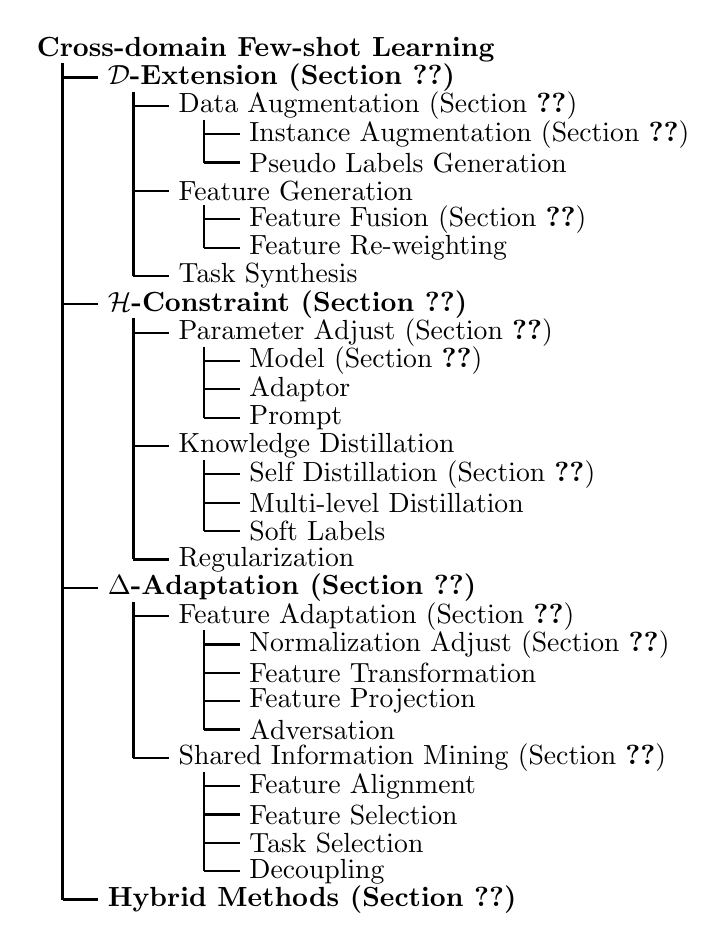
\begin{tikzpicture}[xscale=0.9, yscale=0.36]
\textcolor{black}{
\draw [thick, -] (0, 24) -- (0, 24); \node [right] at (-0.5, 24) {\textbf{Cross-domain Few-shot Learning
}};
\draw [thick, -] (0, 23.5) -- (0, -6);
\draw [thick, -] (0, 23) -- (0.5, 23);\node [right] at (0.5, 23) {\textbf{$\mathcal{D}$-Extension (Section~\ref{instance})}};
\draw [thick, -] (1, 22.5) -- (1, 16);
\draw [thick, -] (1, 22) -- (1.5, 22);\node [right] at (1.5, 22) {Data Augmentation (Section~\ref{sec:FSCIC:dba})};
\draw [thick, -] (2, 21.5) -- (2,20);
\draw [thick, -] (2, 21) -- (2.5, 21);\node [right] at (2.5, 21) {Instance Augmentation (Section~\ref{sec:FSCIC:dba:drbm})};
%\draw [thick, -] (2, 20.5) -- (2,19);
\draw [thick, -] (2, 20) -- (2.5, 20);\node [right] at (2.5, 20) {Pseudo Labels Generation};
\draw [thick, -] (1, 19) -- (1.5, 19);\node [right] at (1.5, 19) {Feature Generation
};
\draw [thick, -] (2, 18.5) -- (2,17);
\draw [thick, -] (2, 18) -- (2.5, 18);\node [right] at (2.5, 18) {Feature Fusion (Section~\ref{sec:FSCIC:dba:drbm})};
%\draw [thick, -] (2, 20.5) -- (2,19);
\draw [thick, -] (2, 17) -- (2.5, 17);\node [right] at (2.5, 17) {Feature Re-weighting};
\draw [thick, -] (1, 16) -- (1.5, 16);\node [right] at (1.5, 16) {Task Synthesis
};
\draw [thick, -] (0, 15) -- (0.5, 15);\node [right] at (0.5, 15) {\textbf{$\mathcal{H}$-Constraint (Section~\ref{hypothesis})}};
\draw [thick, -] (1, 14.5) -- (1, 6);
\draw [thick, -] (1, 14) -- (1.5, 14);\node [right] at (1.5, 14) {Parameter Adjust (Section~\ref{sec:FSCIC:dba})};
\draw [thick, -] (2, 13.5) -- (2,11);
\draw [thick, -] (2, 13) -- (2.5, 13);\node [right] at (2.5, 13) {Model (Section~\ref{sec:FSCIC:dba:drbm})};
%\draw [thick, -] (2, 20.5) -- (2,19);
\draw [thick, -] (2, 12) -- (2.5, 12);\node [right] at (2.5, 12) {Adaptor};
\draw [thick, -] (2, 11) -- (2.5, 11);\node [right] at (2.5, 11) {Prompt};
\draw [thick, -] (1, 10) -- (1.5, 10);\node [right] at (1.5, 10) {Knowledge Distillation
};
\draw [thick, -] (2, 9.5) -- (2,7);
\draw [thick, -] (2,9) -- (2.5, 9);\node [right] at (2.5, 9) {Self Distillation (Section~\ref{sec:FSCIC:dba:drbm})};
%\draw [thick, -] (2, 20.5) -- (2,19);
\draw [thick, -] (2, 8) -- (2.5, 8);\node [right] at (2.5, 8) {Multi-level Distillation};
\draw [thick, -] (2, 7) -- (2.5, 7);\node [right] at (2.5, 7) {Soft Labels};
\draw [thick, -] (1, 6) -- (1.5, 6);\node [right] at (1.5, 6) {Regularization
};
\draw [thick, -] (0, 5) -- (0.5, 5);\node [right] at (0.5, 5) {\textbf{$\Delta$-Adaptation (Section~\ref{adaptation})}};
\draw [thick, -] (1, 4.5) -- (1, -1);
\draw [thick, -] (1, 4) -- (1.5, 4);\node [right] at (1.5, 4) {Feature Adaptation (Section~\ref{sec:FSCIC:dba})};
\draw [thick, -] (2, 3.5) -- (2,0);
\draw [thick, -] (2, 3) -- (2.5, 3);\node [right] at (2.5, 3) {Normalization Adjust (Section~\ref{sec:FSCIC:dba:drbm})};
%\draw [thick, -] (2, 20.5) -- (2,19);
\draw [thick, -] (2, 2) -- (2.5, 2);\node [right] at (2.5, 2) {Feature Transformation};
\draw [thick, -] (2, 1) -- (2.5, 1);\node [right] at (2.5, 1) {Feature Projection};
\draw [thick, -] (2, 0) -- (2.5, 0);\node [right] at (2.5, 0) {Adversation
};
%\draw [thick, -] (2, -0.5) -- (2,-2);
\draw [thick, -] (1,-1) -- (1.5, -1);\node [right] at (1.5, -1) {Shared Information Mining (Section~\ref{sec:FSCIC:dba:drbm})};
\draw [thick, -] (2, -1.5) -- (2,-5);
\draw [thick, -] (2, -2) -- (2.5, -2);\node [right] at (2.5, -2) {Feature Alignment};
\draw [thick, -] (2, -3) -- (2.5, -3);\node [right] at (2.5, -3) {Feature Selection};
\draw [thick, -] (2, -4) -- (2.5, -4);\node [right] at (2.5, -4) {Task Selection};
\draw [thick, -] (2, -5) -- (2.5, -5);\node [right] at (2.5, -5) {Decoupling};
\draw [thick, -] (0, -6) -- (0.5, -6);\node [right] at (0.5, -6) {\textbf{Hybrid Methods (Section~\ref{hybrid})}};}
\end{tikzpicture}}
\vspace{-10pt}
\caption{\textcolor{black}{The taxonomy of representative methods in CDFSL.}}
\label{out}
\end{figure}
%\end{wrapfigure}
\fi
\section{Multi-Site Physiological Monitoring Dataset}
\label{sec:dataset}

We collected a large dataset of subjects seated in front of a video camera with several attached contact PPG sensors. Subjects were instructed to avoid wearing clothes that obstructed the arms and legs. A sample video frame is shown in Fig.~\ref{fig:teaser}, where the subject's face, arms, and legs are visible simultaneously. To the authors' knowledge, this is the first dataset that allows for simultaneous ground truthed rPPG at more than two sites on the body.

The collection began with the subject holding their left hand upright facing the camera for 90 seconds. This allows for evaluation of rPPG on the palm, a region with glabrous skin that is valuable for remote pulse estimation~\cite{Cao2023}. For the remainder of the session, subjects underwent a blood pressure measurement, guided breathing exercise, and relaxation period. On average, the sessions evaluated in this paper last for approximately 5.7 minutes.

\subsection{Apparatus}
Video of the full subject was recorded with a DFK 33UX290 RGB camera from The Imaging Source (TIS). Raw video was recorded at 90 FPS with a resolution of 1920 $\times$ 1080 pixels. To record blood oxygenation (SpO2) and pulse rate, we collected 60 samples per second from an FDA-certified Contec CMS50EA pulse oximeter attached to an index finger. To support research in pulse transit time, we attached nine MAX30101 contact PPG sensors that recorded red and near-infrared signals at 400 samples per second. Each leg and arm had two attached sensors via elastic straps, and the last sensor was attached to the back of the neck with medical tape. All sensors and the camera recorded raw data to a single collection machine with the associated timestamps for easy synchronization.

\subsection{Data Preprocessing}
To properly evaluate rPPG approaches, we created a global pulse rate estimate from the multiple contact sensors. Contact PPG signals recorded from the nine sites with the MAX30101 sensors contain varying levels of noise throughout the session depending on body movements. However, the pulse signal is likely present in at least one signal at any given point in time, since movements may be isolated to local regions.

Using this assumption, we combined the multiple pulse signals using a sliding window approach and bandpass filtering. We relied on the FDA-certified CMS50EA oximeter's pulse rate estimate to define the bounds of a narrow bandpass filter for the MAX30101 signals. Given the estimated pulse rate from the fingertip oximeter $Y$, we specified a padding around this value, $\Delta Y = 30$ bpm, and filtered the MAX30101 signals with a 2nd order Butterworth filter with lower and upper cutoffs of $Y - \Delta Y$ and $Y + \Delta Y$, respectively.

\begin{figure}
    \centering
    \includegraphics[width=\linewidth]{figures/ground_truth_preprocessing.pdf}
    \caption{Processing of the contact PPG waveforms to produce a robust pulse rate. (a) The z-normalized waveforms from all sensors. (b) Bandpass filtered signals around the fingertip oximeter's pulse rate $\pm$ 30 bpm. (c) The signals were added together and the envelope is calculated. (d) The combined signal was divided by the envelope.}
    \label{fig:ground_truth}
\end{figure}

Specifically, for a sliding 10-second window with a stride of a single sample at 400 Hz, the waveforms underwent z-normalization, followed by filtering around the fingertip oximeter's pulse rate, then they were summed together into the combined waveform for that window. Finally, we divided the complete combined waveform by its envelope, which was calculated from the Hilbert transform. The process for signal combination is shown in Fig.~\ref{fig:ground_truth}. In the figure, between seconds 2 and 5, there appears to be noise from motion in multiple sensors, but the combined signal in subplot (d) remains clean.

\section{Multi-Site rPPG Approach}
\label{sec:approach}
Our pipeline to perform remote pulse estimation on our MSPM dataset consists of preprocessing, signal extraction and pulse rate estimation. We applied three pulse estimation algorithms: a chrominace-based method using color difference signals (CHROM)~\cite{DeHaan2013}, plane-orthogonal-to-skin tone (POS)~\cite{Wang2017}, and a 3D-CNN deep learning method RPNet~\cite{Speth_CVIU_2021}. These three methods perform well for both stationary and moving subjects, which are characteristic of our MSPM dataset. The RPNet model was trained on face videos from the large and challenging deception detection and physiological monitoring dataset (DDPM)~\cite{Speth_IJCB_2021,Vance2022}. The model was not fine-tuned on any data from MSPM, so we tested how well the model could transfer to new subjects, lighting, standoff, and movement. Since the model was only trained on cropped faces, we also investigated its ability to transfer to spatially dissimilar regions such as the arms and legs. One of the benefits of CHROM and POS is that they do not have any spatial priors and only expect RGB traces from skin pixels.

\subsection{Preprocessing}
\subsubsection{ROI selection}\label{sec:ROI}
Given skin pixels including face, arms, and legs collected by MSPM, we selected these five different body parts as our ROIs. We applied Self-Correction Human Parsing (SCHP)~\cite{li2020self} for body segmentation to the eighty-seven subjects of MSPM. Frame (b) of Fig.~\ref{fig:frames} shows masks of the twenty parts from SCHP for a single frame. Masked skin pixels of each ROI were averaged and supplied to CHROM and POS for signal extractions. For each masked ROI, we also calculated the minimum and maximum values of $(x, y)$ locations of each mask to form bounding boxes for RPNet. Similarly, we created bounding boxes for palms using four key points of the palm generated by Mediapipe Hand detection~\cite{Zhang2020MPHands}. Frame (c) of Fig.~\ref{fig:frames} shows the bounding box for the palm.

\subsubsection{Human Key Points Detection}
To better investigate rPPG performance, we applied Mediapipe Pose detection~\cite{Bazarevsky2020} to detect key points of the human skeleton for local error estimation of the whole body (described later in Sec. \ref{sec:local}). There are thirty-three key points in total which define locations of many of the body's joints, including detailed locations for hands. 
Frame (d) of Fig.~\ref{fig:frames} shows an example of the skeleton detection results.

\subsection{Signal Extraction}
\subsubsection{Color Transformation Methods}

For each body part, we calculated spatial averages of skin pixels to reduce camera quantization error and generate 1D signals for each channel of RGB. CHROM~\cite{DeHaan2013} and POS~\cite{Wang2017} combined the signals of the three channels linearly to remove noise from movement or lighting to generate more robust pulse signals.

\setlength\tabcolsep{3.9pt}
\begin{table*}[htb!]
\caption{Pulse rate estimation results. MAE: Mean Absolute Error; $r$: Pearson correlation coefficient.}
\fontsize{9.0}{9}\selectfont
\centering
\begin{tabular}{l cc cc cc cc cc | cc | cccc}
\toprule
& \multicolumn{10}{c|}{Both relaxed and hand raise} & \multicolumn{2}{c|}{Relaxed} & \multicolumn{4}{c}{Hand raise}\\
\cmidrule(lr){2-11}\cmidrule(lr){12-13}\cmidrule(lr){14-17}
\multirow{3}{*}{\begin{tabular}[c]{@{}l@{}}\\Methods\end{tabular}} &
\multicolumn{2}{c}{Face} &
\multicolumn{2}{c}{Right leg} &
\multicolumn{2}{c}{Left leg} &
\multicolumn{2}{c}{Right arm} &
\multicolumn{2}{c|}{Left arm} &
\multicolumn{2}{c|}{Left arm} &
\multicolumn{2}{c}{Left arm} &
\multicolumn{2}{c}{Palm}\\ 
\cmidrule(lr){2-3}
\cmidrule(lr){4-5}
\cmidrule(lr){6-7}
\cmidrule(lr){8-9}
\cmidrule(lr){10-11}
\cmidrule(lr){12-13}
\cmidrule(lr){14-15}
\cmidrule(lr){16-17}
& \begin{tabular}[c]{@{}c@{}}MAE\\ (bpm)\end{tabular} & $r$
& \begin{tabular}[c]{@{}c@{}}MAE\\ (bpm)\end{tabular} & $r$
& \begin{tabular}[c]{@{}c@{}}MAE\\ (bpm)\end{tabular} & $r$
& \begin{tabular}[c]{@{}c@{}}MAE\\ (bpm)\end{tabular} & $r$
& \begin{tabular}[c]{@{}c@{}}MAE\\ (bpm)\end{tabular} & $r$
& \begin{tabular}[c]{@{}c@{}}MAE\\ (bpm)\end{tabular} & $r$
& \begin{tabular}[c]{@{}c@{}}MAE\\ (bpm)\end{tabular} & $r$
& \begin{tabular}[c]{@{}c@{}}MAE\\ (bpm)\end{tabular} & $r$\\
\midrule
CHROM \cite{DeHaan2013} &
    2.38  & 0.85 &
    10.92 & 0.42 &
    11.07 & 0.41 &
    9.13  & 0.50 &
    9.81  & 0.41 &
    11.57 & 0.35 &
    4.26  & 0.71 &
    5.01  & 0.67 \\
POS \cite{Wang2017} &
    \textbf{1.38} & \textbf{0.93} &
    \textbf{6.96} & \textbf{0.54} &
    \textbf{7.11} & \textbf{0.54} &
    \textbf{3.60} & \textbf{0.78} &
    \textbf{6.04} & \textbf{0.64} &
    \textbf{6.88} & \textbf{0.61} &
    \textbf{3.40} & \textbf{0.75} &
    \textbf{3.88} & \textbf{0.76} \\
RPNet \cite{Speth_CVIU_2021}\tnote{\textdagger} &
    2.27  & 0.87 &
    29.50 & 0.14 &
    30.42 & 0.11 &
    23.94 & 0.15 &
    23.15 & 0.16 &
    27.01 & 0.11 &
    11.06 & 0.38 &
    6.70  & 0.52 \\
\bottomrule
\end{tabular}
\label{tab:within_dataset}
\end{table*}

\subsubsection{Learning-Based Method}
We used the generated bounding box coordinates to crop ROIs from each frame for each body part and downsized these ROIs to 64x64 pixels using bicubic interpolation. The RPNet model we used was trained on the DDPM dataset~\cite{Speth_IJCB_2021,Vance2022} where the frame rate is 90 frames per second (fps), which is the same as our MSPM dataset. The trained RPNet model was fed video clips of 135 frames (1.5 seconds) as described in the original paper~\cite{Speth_CVIU_2021}.

\subsection{Filtering and Pulse Rate Calculation}
Remote pulse estimation over non-face regions is challenging, because of their lower signal-to-noise ratio than the face. To improve signal quality for all approaches, we applied a 4th order Butterworth bandpass filter with cutoff frequencies of 40 bpm and 180 bpm. Bandpass filtering was not used in the original POS and RPNet implementations, but we found the POS estimates in particular to contain high frequency noise before filtering. To compute the dominant pulsatile component in the rPPG waveforms, we applied the short-time Fourier transform (STFT) over a sliding 10-second window (900 frames in our videos), and selected the spectral peak as the pulse rate.


\section{Global rPPG Experiments}
\label{sec:global}
\subsection{Global Evaluation}
We refer to rPPG with all pixels in a region of interest as ``global" rPPG. We evaluated global rPPG performance over the face, arms, and legs with the color transformation approaches (CHROM~\cite{DeHaan2013} and POS~\cite{Wang2017}), and a 3D-CNN approach (RPNet~\cite{Speth_CVIU_2021}). We compared the rPPG quality by evaluating the pulse rate performance. We applied the same method for pulse rate estimation on both the ground truth signals and the rPPG signals for fair evaluation~\cite{Mironenko2020}. 
We used popular error metrics to compare the pulse rate estimates, including mean absolute error (MAE) and Pearson's correlation coefficient ($r$).

\subsection{Global Results}

The results of global rPPG experiments with different body parts are shown in Table~\ref{tab:within_dataset}. We show results for the entire sequence as well as for separate components in which the left arm is either relaxed or raised with left palm frontally presented. We observed the best MAE and $r$ for the face region. CHROM and RPNet give similar performance on the face region, with RPNet giving slightly better performance. RPNet performed poorly on the non-face regions, however, likely indicating that the model has learned spatial priors to look for facial features. Additionally, the deep learning model may be overfit to the skin thickness, melanin concentration, and microcirculation present in the glabrous skin of the face. The improved performance for RPNet on the palm (also with glabrous skin) helps justify this explanation.

The POS algorithm gives the best performance for all body regions in terms of both MAE and $r$. This is especially impressive given that it is a simple linear method. It also shows that color changes from blood volume are similar over different skin thicknesses and underlying microvasculature. For POS and CHROM, the order of performance from best to worst is face, arms, then legs. The palm also gives good performance for all approaches, due to physical similarities to the skin on the face.

Figure \ref{fig:result_waveforms} shows predicted waveforms from a 10-second window for the same subject at different locations. The nearest contact PPG waveforms are bandpass filtered and plotted against the predictions to show that many of the predictions contain the underlying dominant pulse even in the presence of higher frequency noise. The difference in waveform morphology across body location shows how informative full-body rPPG can be. For this particular segment, the legs contain a strong second harmonic, which may arise from either the closure of the aortic valve during forward wave propagation, or wave reflections occurring at structural discontinuities along the femoral arteries~\cite{London1999}. Future studies on this dataset will explore different waveform morphologies at a finer scale and their relation to arterial stiffness and blood pressure.

Figure~\ref{fig:result_HRs} shows pulse rates calculated from POS predictions over the entire session for 3 subjects. Interestingly, the errors generally occur as spikes of short duration rather than sustained periods of large offset. Even for the left arm, which is the worst-performing region for subject 0, the errors appear to be due to short periods where the second harmonic contains more power than the first harmonic. It is possible that simple heuristics during postprocessing could remove these transient errors. In general, the global POS signals give meaningful predictions for most applications, even in non-face regions.

\begin{figure}
    \centering
    \includegraphics[width=\linewidth]{figures/results/wave.pdf}
    \caption{Pulse waveform predictions from POS overlayed with the nearest contact-PPG waveforms for a 10 second window.}
    \label{fig:result_waveforms}
\end{figure}

\begin{figure}
    \centering
    \includegraphics[width=\linewidth]{figures/results/HR_3.pdf}
    \caption{Pulse rate predictions from POS for 3 subjects over the course of a full session compared to the ground truth.}
    \label{fig:result_HRs}
\end{figure}

\section{Local rPPG Experiments}
\label{sec:local}

\subsection{Local Evaluation}
In addition to analyzing performance for the entire face, arm, and legs, we performed a ``local" analysis on subregions of pixels in the native video resolution. This gives a more detailed evaluation on rPPG quality over the visible skin on the body. We selected POS~\cite{Wang2017} as the rPPG method, since it was the best performing for each of the global regions.

We used the ROIs described in section~\ref{sec:ROI} to define bounds for a non-overlapping sliding window of 20x20 pixel subregions. The POS algorithm was applied on 10-second non-overlapping time windows of the spatially averaged subregions for the whole video. The predictions were then linearly interpolated up to the native image resolution (i.e. 20 times as large along the x- and y-axes). Next, we computed error metrics at each pixel location for the 10-second windows, which results in 9 error frames for the hand raising portion, and around 25 error frames for the sitting portion per subject.

For error metrics we used MAE between the predicted and ground truth pulse rate and signal-to-noise ratio (SNR). The SNR was calculated similarly to \cite{DeHaan2013,Nowara_BOE_2021}, where the sum of spectral power around the signal bands in the first and second harmonics ($\pm 6$ bpm) was divided by the total power outside the signal bands.

To remove spurious local errors outside of the skin pixel regions, we applied the average SCHP mask (see frame (b) in Fig.~\ref{fig:frames}) for the time window to the error frames. Since subjects sat in slightly different positions throughout the interview, we aligned each body part across subjects for an accurate physiological error map. To do this we used the pose keypoints from Mediapipe (see frame (d) in Fig.~\ref{fig:frames}). We first calculated the average pose across all subjects for the hand raising and relaxed portions as the target poses. Then for each error frame for every subject, we applied a homographic transformation from the time window's pose to the hand raising or relaxed portion's target pose.

\begin{figure*}
    \centering
    \includegraphics[width=0.85\linewidth]{figures/heatmaps/heatmaps_pagewidth_dehaan_harm.pdf}
    \caption{A heatmap of the local POS signal quality across the visible skin. POS signals are predicted over 20x20 pixel subregions, masked with SCHP~\cite{li2020self}, and the human pose is aligned with a homographic transformation.}
    \label{fig:heatmap}
\end{figure*}

\subsection{Local Results}
Figure~\ref{fig:heatmap} shows a heatmap of local pulse estimation performance for the POS algorithm. The hand raising and sitting portions are visualized separately, since the body positions were much different. In general, we found the face to hold the strongest rPPG signal. In the hand raising heatmap, we can see that the palm gave relatively low errors compared with the arms and legs. This supports the hypothesis that signal quality is higher on glabrous than non-glabrous skin~\cite{Cao2023}, and shows promise for substituting the face region with the hand if necessary.

It is useful to analyze each body part separately to assess the signal quality. Firstly, the face appears to give low MAE and high SNR in all regions except the eyes and mouth. This is in line with past research that mainly utilizes the forehead and cheek regions. The arms give relatively low signal quality, but there is a slight improvement visible above the forearm over other regions in the SNR plots. The legs give perhaps the weakest rPPG signal as evidenced by the global results in Table \ref{tab:within_dataset}. Within the local analysis, we can see that the thighs give higher SNR than the shins. This could be due to the thigh's closer proximity to the illuminators, whereas the shins are visibly darker in the video.

In both the hand raising and relaxed portions, the hand gives the second best SNR. In nearly all cases the subject's right hand was resting with the palm facing downwards, indicating that the back of the fingers and hand on non-glabrous skin is still feasible for rPPG. During the hand raising, we see that the signal quality is high on the glabrous skin of the palm. With more sophisticated methods for aligning each subject's palms, we believe the error maps would give even higher signal quality.
\section{Pulse Transit Time Experiments}
\label{sec:ptt}

\begin{figure*}
        \centering
        \begin{minipage}[t]{0.37\linewidth}
        \begin{subfigure}{\linewidth}
        \includegraphics[width=\linewidth]{figures/PTT_subfig.pdf}
        \caption{}
        \label{subfig:ptts}
        \end{subfigure}
        \end{minipage}
        \hfil
        \begin{minipage}[t]{0.25\linewidth}
        \begin{subfigure}{\linewidth}
        \includegraphics[width=\linewidth]{figures/PTT_POS_subfig.pdf}
        \vspace{7.27em}
        \caption{}
        \label{subfig:rptts}
        \end{subfigure}
        \end{minipage}
        \hfil
        \begin{minipage}[t]{0.37\linewidth}
        \begin{subfigure}{\linewidth}
        \includegraphics[width=\linewidth]{figures/PTT_boxplots_horizontal_30.pdf}
        \caption{}
        \label{subfig:ptt_boxplots}
        \end{subfigure}
        \end{minipage}
    \caption{Pulse transit time from both contact PPG and rPPG calculated by a sliding cross-correlation between pairs of waveforms. (a) Time lags between the MAX30101 contact PPG sensors. (b) Time lags between POS waveform predictions on the five different body regions. (c) Grouped boxplots comparing the pulse transit time from PPG and rPPG. For the PPG measurements on the arms and legs we only used the forearm and knee sensors, respectively. The PTT is calculated as $X-Y$ given a label of measurement sites ``$X$ to $Y$".}
    \label{fig:ptts}
\end{figure*}

\subsection{Pulse Transit Time for Contact PPG Sensors}
Contact PPG measurements at different sites on the body contain small phase offsets due to different proximities to the heart. These offsets are sometimes referred to as differential pulse transit times (dPTT)~\cite{Block2020} and are negatively correlated with blood pressure. Throughout the paper we treat PTT and dPTT interchangeably. When fusing the PPG measurements at multiple sites into a single ground truth, we summed the waveforms without applying a phase shift. To justify this simplification, we calculated the differential pulse transit time between all pairs of sensors. Fig. \ref{subfig:ptts} shows a heatmap of the phase offsets between all pairs of PPG signals in milliseconds.

The phase differences were calculated with a sliding cross-correlation. We used a window size of 5 seconds (2,000 points) with a stride of 10 milliseconds (4 points), and a maximum lag 300 milliseconds, which is much higher than a typical transit time~\cite{Block2020}.
The sliding cross-correlation approach for PTT analysis is simple, but could be improved in future work by using foot-finding methods that measure time differences at the diastolic foot~\cite{Mukkamala2015}. 
The index with the maximum correlation was selected as the phase shift for each window. All pairs of transit times formed a skew-symmetric matrix, where $A^T = -A$.

In general, the phase offset between different sites is quite small relative to the pulse rate frequency. For example, the largest average phase offset of 51 milliseconds occurs between the left tricep and the right ankle. Given even a high pulse rate of 180 bpm, the phase angle for such a shift is only 27.66 degrees. Since most phase offsets are lower, there is very little risk of interference when summing the waveforms. The pulse transit times provide interesting physiological measurements of blood flow throughout the body. As mentioned previously, the largest difference occurs between the triceps and ankle. The triceps receive blood faster via the brachial artery and a closer proximity to the aorta than the lower legs. We had originally theorized that the neck sensor would sense the pulse wave before the other sensors, but our analysis refutes this.


\subsection{Pulse Transit Time from rPPG}
Beyond the benefit of contactless monitoring, one of the most powerful properties of a camera is the ability to sense at multiple spatial locations. To leverage this, we performed remote pulse transit time (rPTT) with a sliding cross-correlation from the POS rPPG waveforms at multiple sites on the body. The POS waveforms are noisier than the PPG waveforms in the legs and arms, but the infrequent pulse rate errors (see Fig. \ref{fig:result_HRs}) indicate that the signal quality is high enough for rPTT.

Figure \ref{subfig:rptts} shows a heatmap of the rPTT between all pairs of the face, legs, and arms. The maximum observed rPTT is 46.75 ms between the face and left leg, which is within a reasonable range compared to the largest contact-PTT measurements between triceps and legs (51.23 ms and 48.82 ms). An interesting observation is the bilateral asymmetry visible in the rPTT left and right sides of the body. The pulse waves from the right side of the body were consistently observed sooner than the left side of the body.

To compare the rPTT measurements with the PPG-derived PTT values we selected the nearest contact sensors to the rPTT measurement sites, and discarded the rest (\eg ankles and triceps). Figure \ref{subfig:ptt_boxplots} shows boxplots of the PTT values for all 5-second time windows in the relaxation portion of the dataset. The groups were sorted by the median PTT at the pair of measurement sites for easier viewing. The means of the rPTT measurements via POS are not perfectly aligned with the PTTs --- but upon further inspection, we can see that rPTT and PTT correlate well across the pairs of body sites. A potential reason for the bias in the rPTT values is that the signal quality is not uniform over the measured body sites. For example, the POS signal on the arms is likely shifted in phase towards the pulse wave at the hands. Similarly, the POS wave is likely shifted more towards the phase of the thighs than the lower legs. Furthermore, the sampling rate of the video is 90 fps, so large time lags such as 55 ms will only occur as 5 frames. Future work will perform more robust transit time calculations via the systolic foot and finer-grained spatial measurements of rPTT to better align with the contact-PPG sensors.

\section{Conclusions}
We proposed a novel non-contrastive learning approach for end-to-end unsupervised signal regression, with specific experiments on blood volume pulse estimation from face videos.
This SiNC framework effectively learns powerful visual features with only loose frequency constraints.
We demonstrated this by training accurate rPPG models using non-rPPG data and our simple loss functions.
Given the subtlety of the rPPG signal, we believe our work can be extended to other signal regression tasks in the domain of remote vitals estimation.
\section*{Acknowledgements}
This research was sponsored by the Securiport Global Innovation Cell, a division of Securiport LLC. Commercial equipment is identified in this work in order to adequately specify or describe the subject matter. In no case does such identification imply recommendation or endorsement by Securiport LLC, nor does it imply that the equipment identified is necessarily the best available for this purpose. The opinions, findings, and conclusions or recommendations expressed in this publication are those of the authors and do not necessarily reflect the views of our sponsors.


%%%%%%%%% REFERENCES
{\small
\bibliographystyle{ieee_fullname}
\bibliography{egbib}
}

\end{document}
